\chapter{Perifer interaktion}
\label{PeriferInteratkion}
%
Skriv en hat for hele kapitlet
%
\begin{itemize}
  \item Hvorfor er det interesant at designe produkter, som kan reagere på perifer interaktion? (fordele og ulemper) 
  \item Socialt acceptabelt 
  \item Adfærdsændringer
\end{itemize}
\noindent
%
Perifer interaktion er ikke nyt. Vi gør det alle sammen, når vi i løbet af vores dagligdag foretager adskillige aktiviteter i vores perifere opmærksomhed, \parencite[s. 1]{PDF:PeripheralInteraction}. Det forudsætter dog at disse perifere interaktioner primært retter sig mod ikke-computer-relateret aktiviteter, såsom at føre en samtale imedens der laves mad. Rettes fokus derimod til \textit{Human-Computer-Interaction}, HCI, så forlanger diverse elektroniske apparater vores centrale opmærksomhed ved at blinke, ringe og vibrere, \parencite[s. 1]{PDF:PeripheralInteraction}. Ifølge \textcite[s. 3]{PDF:PeripheralInteraction} så bevæger interaktionen med elektroniske apparater sig uforudsigeligt mellem den centrale og perifere opmærksomhed, i modsætning til ikke-computer-relateret aktiviteter, som i større grad kan kontrolleres. Grunden til at disse apparater frit kan bevæge sig fra den perifere til den centrale opmærksomhed skyldes, at vi sjælendt har kontrol over hvornår et apparat kræver den centrale opmærksomhed. Så snart et elektronisk apparat befinder sig i den centrale opmærksomhed, så vil ens opmærksomhed midlertidigt fjernes fra den primære opgave, indtil interaktionen med apparatet er afsluttet. Konsekvenserne af at blive forstyrret og skulle rette opmærksomheden væk fra ens primære opgave over til apparatet, er en øget kognitiv belastning samt en større risiko for at begå fejl i den primære opgave, \parencite[ss. 188-189][s. 162]{PDF:PeripheralInteraction, PDF:ComparingInputModalities}. 

Istedet for at forstætte med at designe elektroniske apparater, som både kræver den centrale opmærksomhed og kræver at opmærksomheden flyttes væk fra den primære opgave, så bør apparaterne derimod designes så de i højere grad bliver en integreret del af vores daglige rutiner, \parencite[s. 239]{PDF:PICharacteristicsAndConsiderations}. Ved at designe apparater ud fra den tilgang så vil det tillade perifer interaktion, fordi det, blandt andet, bygger på teori omkring delt-opmærksomhed. Ifølge disse teorier råder mennesket over en bestemt mængde af mentale resourcer, som afhængigt af opgavernes sværhedsgrad, frit kan distribueres mellem opgaverne, \parencite[s. 240]{PDF:PICharacteristicsAndConsiderations}. Derudover tillader delt-opmærksomhed også at flere aktiviteter kan foretages samtidigt, så længe de kun kræve få mentale ressourcer, \parencite[s. 2]{PDF:FacilitatingPIDesignAndEvaluation}. Så istedet for at elektroniske apparater kræver den fulde opmærksomhed, så er det ved perifer interaktion muligt at distribuere sin opmærksomhed for på den måde at foretage flere aktivitet samtidig. Hvis interaktion med computere og andre elektroniske apparater blev flyttet til det perifere kan det, ifølge \textcite[s. 11]{PDF:TheComputerWeiser}, potentielt være med til at fremme det sociale samvær, som der eksempelvist er på arbejdsmarkedet. Derudover pointerer \textcite[s. 11]{PDF:TheComputerWeiser} at de elektroniske apparater skal tilpasses til den menneskelige hverdag og ikke omvendt. Ligeledes bør der tages højde for at desto flere elektroniske apparater, der produceres til at fange vores centrale opmærksomhed, desto større er behovet for at en del af interaktionen bliver perifer, \parencite[s. 240]{PDF:PICharacteristicsAndConsiderations}. \blankline
%
Behovet for at designe elektroniske apparater, som tillader perifer interaktion er ikke nyt. Allerede i halvfemserne blev der af \textcite[s. 3]{PDF:TheComingAgeOfCalmTech} efterspurgt, at såfremt apparaterne skulle være allevegne, så skal de ikke være i vejen. I den forbindelse blev \textit{Calm Technology} skabt. Principperne bag \textit{Calm Technology} er simple; ved at allokere noget af interaktionen til det perifere er det muligt, at håndtere flere informationer ad gangen. Derudover vil denne allokering give en følelse af kontrol, fordi det er muligt selv at kontrollere hvornår noget er i den centrale kontra den perifere opmærksomhed, \parencite[s. 4]{PDF:TheComingAgeOfCalmTech}. Udover perifer interaktion, som blandt andet bygger på \textit{Calm Technology}, tyder det på at der også kan drages nytte af \textit{Casual Interaction}. Ifølge \textcite[ss. 118-119]{PDF:PeripheralInteraction} vedrører \textit{casual interaction} hvor meget kontrol, der overdrages til et elektronisk apparat. Med \textit{casual interaction} er det muligt at designe apparater, som kan interageres med over en større afstand, som kræver færre kognitive resourcer, som kan interageres med ved hjælp af andre objektet og som kan interageres med uden stor præcision, \parencite[s. 128]{PDF:PeripheralInteraction}        
%
\begin{figure}[H]
	\centering
	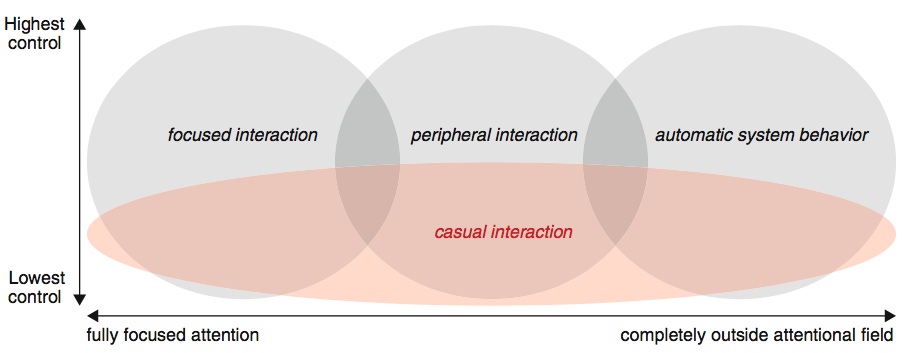
\includegraphics[resolution=300,width=\textwidth]{LevelsOfInteraction}
	\caption{Sammenhæng mellem de tre niveauer af interaktion; fokuseret, perifert og automatisk og hvilket niveau af kontrol, der ønskes samt mængden af opmærksomhed,  \parencite[s. 118]{PDF:PeripheralInteraction}.}
	\label{fig:LevelsOfInteraction}
\end{figure}
\noindent
%
Ved alle tre interaktionsniveauer er det muligt at overdrage kontrol til et elektronisk apparat, hvormed interaktionen bliver afslappet, jævnfør \autoref{fig:LevelsOfInteraction}. Det kan gøres både i den centrale, perifere og fuldautomatiske opmærksomhed. Nu hvor størstedelen af de elektroniske apparater er designet til at blive interageret med i den centrale opmærksomhed og tilmed kræver fuld kontrol, \parencite[s. 118]{PDF:PeripheralInteraction}, så må det antages, at det er det vi har vænnet os til. Men hvad så når vi står i situationer, hvor vi ikke er i stand til eller magter at have den fulde kontrol? Ifølge \textcite[s. 123]{PDF:PeripheralInteraction} kan der være tre årsager til at vi er villige til at overdrage kontrol til elektroniske apparater; 1) mentale årsager, 2) fysiske årsager og 3) sociale årsager. Et andet spørgsmål, som \textcite[s. 124]{PDF:PeripheralInteraction} stiller, vedrører om vi overhovedet er villige til at overdrage noget kontrol til de elektroniske apparater? Og svaret er, at så længe opgaven er tilstrækkeligt let og vi stadig har tilstrækkeligt kontrol til at løse opgaven, så ja, så er vi villige til at overdrage kontrol, \parencite[s. 124]{PDF:PeripheralInteraction}.

Udelades \textit{casual interaction} samt niveauet af kontrol, på \autoref{fig:LevelsOfInteraction}, er de resterende elementer; de tre niveauer af interaktion og mængden af opmærksomhed. Ifølge \textcite[s. 6]{PDF:PeripheralInteraction} så bliver perifer interaktion ikke udnyttet i lige så høj grad, som både fokuserede og automatiske interaktion. Til gengæld bliver der i større grad udviklet elektroniske apparater, der understøtter automatisk interaktion, som for eksempel bevægelsessensorer, der automatisk tænder lyset i et rum så snart der registreres en bevægelse, uanset om  hensigten var at tænde lyset, \parencite[s. 5]{PDF:PeripheralInteraction}. 

Det tyder kraftigt på at der findes et stort uudnyttet område, som har et stort potentiale, hvor det er muligt at designe elektroniske apparater, som aflaster de kognitive resourcer, tillader tilstrækkeligt med kontrol og som potentielt kan fremme vores sociale kompetencer. Det er ihvertfald højst relevant, \parencite[s. 239]{PDF:PICharacteristicsAndConsiderations}, og nødvendigt, \parencite[s. 3]{PDF:TheComingAgeOfCalmTech}, at inddrage og udnytte mulighederne med perifer interaktion i fremtidige elektroniske apparater.     





 
